\section{Theoretical Analysis}
\label{sec:analysis}

In this section, the circuit shown in Figure~\ref{fig:rc} is analysed
theoretically.
The key equations for all the theoretical analysis ar shown below:
To compute $`t_on$
\begin{equation}
	V_s/n(t)*C*w*sin(w*t_off) = (1/R1)*(V_s/n)*cos(w*t_off) +  I_x*(e^{12/eta*Vt*k} -1)
\end{equation}

In which $i_D = i_R + i_C$

To compute $t_on$ we use the equation
\begin{equation}
	(V_s/n)*cos(w*t_off) = -(V_s/n)*cos(w*t_off)*(e^{(-1/R_eq*C)*(t_on - T_off)}
\end{equation}


\subsection{envelope detector}

In this section we will start by analyzing the envelope detector, where t varies from 0 to 20 ms, by using the main equations above.
\begin{equation}
	V_6n(t) = V_xe^{-(t)/CR_eq}
\end{equation}

Using octave we obtain the following table:
\begin{table}[h!]
	\centering
	\begin{tabular}{|l|r|}
		\hline    
		{\bf Name} & {\bf Value [mA]} \\ \hline
		DC Level & 12.000000 \\  \hline 
Voltage ripple & 0.000000 \\  \hline 

	\end{tabular}
	\caption{ }
	\label{tab:op}
\end{table}

We can now plot the graph of the solution for t raging from 0 to 20 ms:

\begin{figure}[h!] \centering
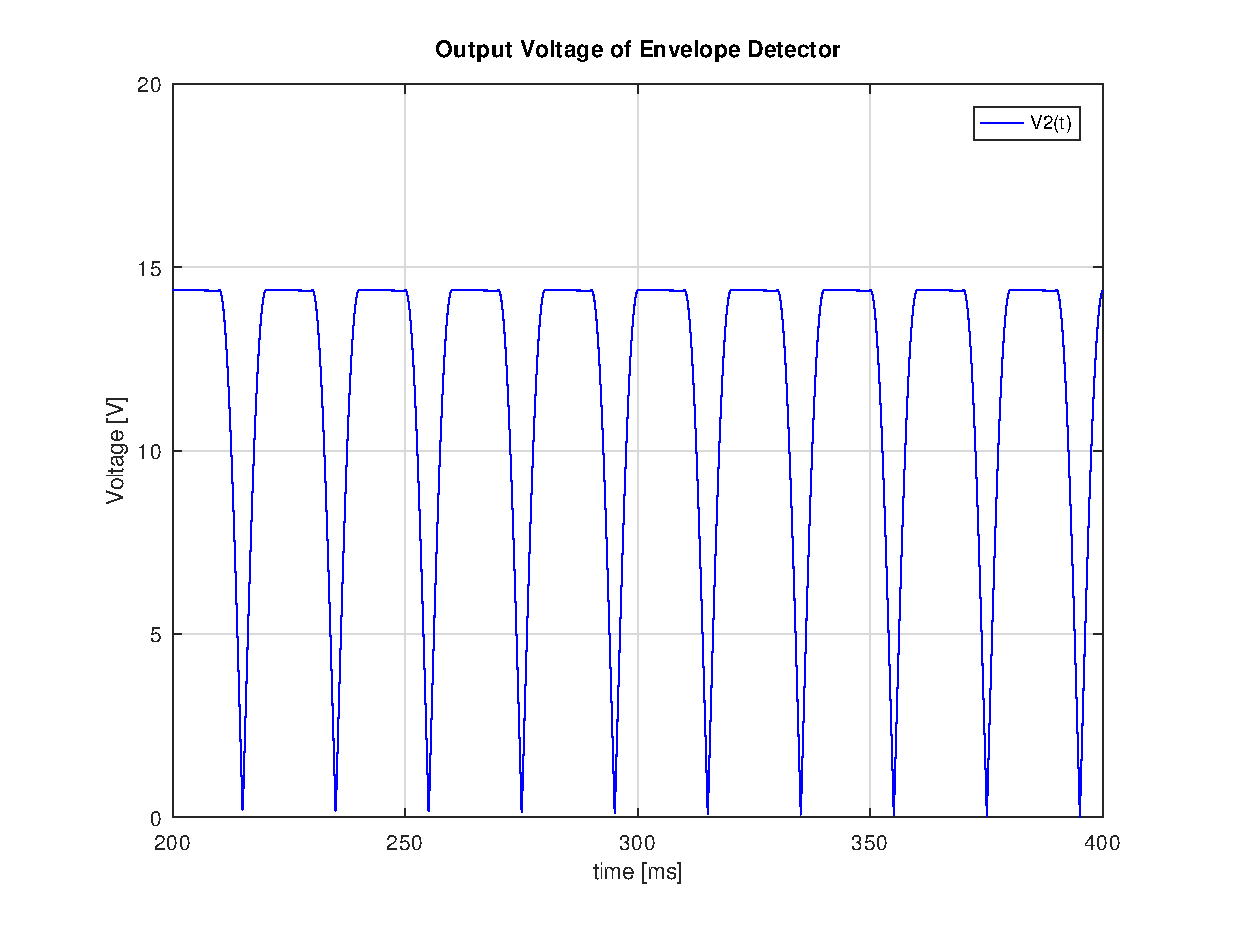
\includegraphics[width=0.6\linewidth]{Output_Envelope_Detector.eps}
\caption{envelop detector output}
\label{fig:rc1}
\end{figure}
	
\subsection{voltage regulator}

The voltage regulator theoretical analysis of this circuit, like with the envelope detector is done with the help of a key equation above.
\begin{equation}
	V_6n(t) = V_xe^{-(t)/CR_eq}
\end{equation}

After this, we can plot the following graphic:
\begin{figure}[h!] \centering
	\includegraphics[width=0.6\linewidth]{Output_Voltage_Regulater.eps}
	\caption{Voltage regulator output}
	\label{fig:rc1}
\end{figure}


\subsection{Voltage regulator deviation}

Lastly, we will analyze the voltage regulator deviation plot, which like in the error subsection of the simulation analysis will give us the deviation in our results.

Considering:
\begin{equation}
	V_c(t) = V_6(t) - V_8(t)
\end{equation} 



The graphics of the voltage deviation is:


\begin{figure}[h!] \centering
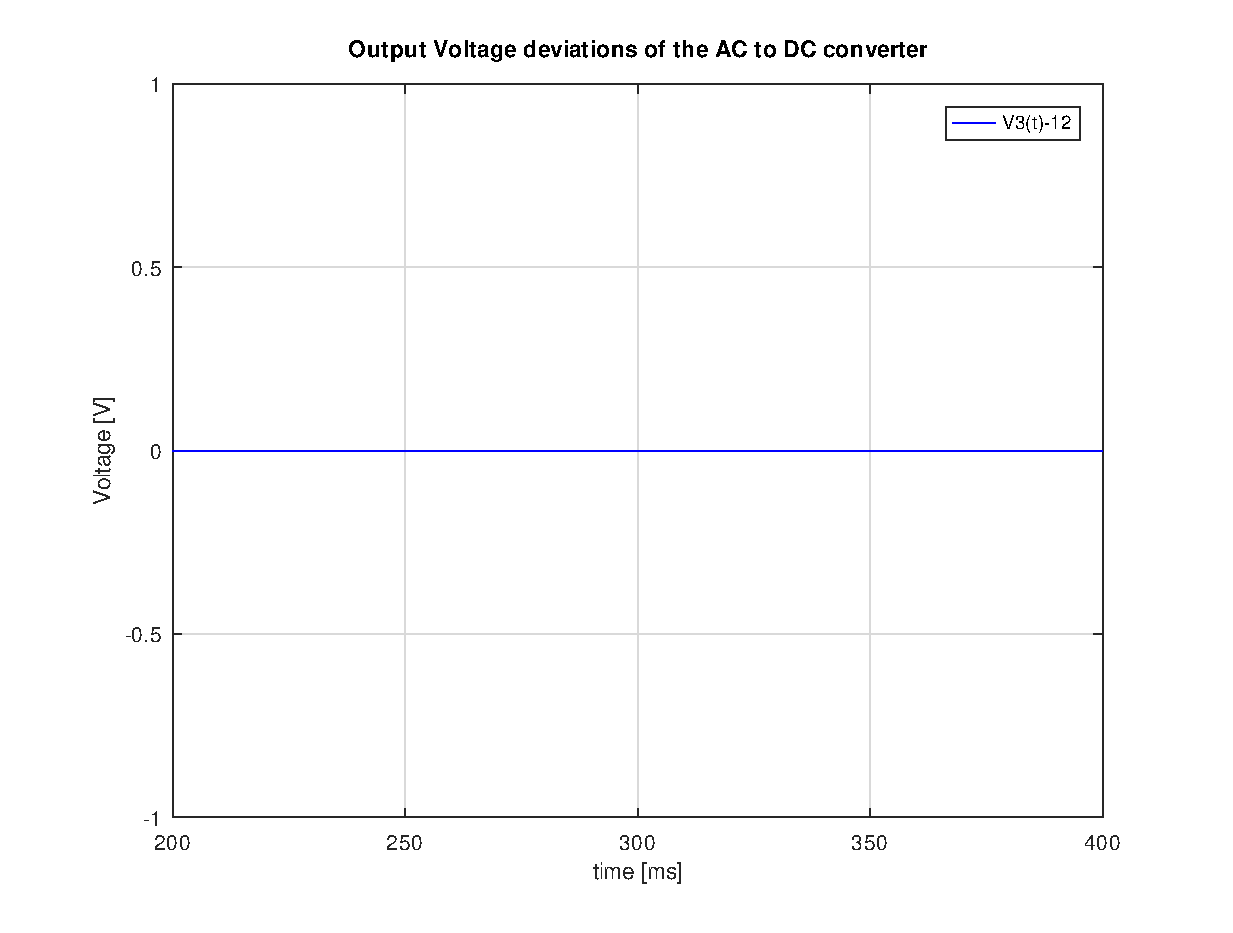
\includegraphics[width=0.6\linewidth]{Output_Voltage_Regulater_deviations.eps}
\caption{Voltage deviation plot}
\label{fig:rc4}
\end{figure}



